\documentclass[a4paper,14pt]{scrreprt}
\usepackage[T1]{fontenc}
\usepackage[utf8]{inputenc}
\usepackage[ngerman]{babel}
\usepackage[table]{xcolor}% http://ctan.org/pkg/xcolor
\usepackage{tabu}
\usepackage{graphicx}
\usepackage{lmodern}
\usepackage{hyperref}\usepackage{geometry}
\geometry{verbose,a4paper,tmargin=22mm,bmargin=45mm,lmargin=30mm,rmargin=30mm}

\begin{document}


%\titlehead{Kopf} %Optionale Kopfzeile
\author{Alexander Rieppel} %Zwei Autoren
\title{Datenbanksynchronisation verteilter Datenbanken} %Titel/Thema
\subject{VSDB} %Fach
\subtitle{Umsetzung mit Couchbase Lite} %Genaueres Thema, Optional
\date{\today} %Datum
\publishers{5AHITT} %Klasse

\maketitle
\tableofcontents
\bibliographystyle{alphadin} 

\chapter{Einf"uhrung}
\section{Umsetzung im Diplomprojekt}
Ziel des Diplomprojektes war es eine Applikation f"ur ein Tablet zu entwickeln, dass die Mitarbeiter der Lebensmittelversuchsanstalt bei der Probennahme im Supermarkt unterst"utzen soll. Insgesamt umfasst das Diplomprojekt eine Android Applikation und eine Server-Applikation. Bei der Probennahme werden Lebensmittel eingekauft, die am Tablet entsprechend in eine Datenbank eingetragen und sp"ater in der LVA f"ur die weiter Bearbeitung bereitgestellt werden. Die Daten werden anschlie"send in die interne Datenbank in der LVA synchronisiert und f"ur die Verarbeitung der Daten durch das Laborteam bereitgestellt. Auf weitere Vorg"ange innerhalb der Firma hat allerdings die Tablet-Applikation keinen Einfluss mehr. Deshalb wird hier lediglich auf den Teil der Speicherung in die Datenbank und vor allem die Synchronisation mit der LVA-Datenbank eingegangen. \\\\Innerhalb der Tablet Applikation wird eine SQLite Datenbank verwendet, da diese nicht sonderlich viele Ressourcen des Tablets ben"otigt und so eine einfache und angenehme Verwendung durch den Benutzer erm"oglicht. Die Datenbank erlaubt zudem nicht allzu viele Datenbanken und im Vergleich zur klassischen MySQL L"osung nur wenige Nutzer. Auf dem firmeneigenen Server l"auft eine klassische Mysql Instanz. Der Auftraggeber hatte zwar die Wahl offen gelassen welche Datenbankl"osung bevorzugt wird, allerdings gleichzeitig auch bekanntgegeben, dass bereits eine Lizenz f"ur Mysql vorhanden ist. Weitere in Betracht gezogene Datenbanksysteme waren PostgreSQL und ebenfalls auch f"ur das Serverprogramm SQLite. \\\\ Die Umsetzung sah so aus, dass Daten vom Tablet zun"achst an die Server-Applikation "uber Java-Streams versandt und anschlie"send von der Server-Applikation entsprechend in die Datenbank eingepflegt werden. W"ahrend Daten von der Datenbank auf das Tablet synchronisiert sind, d"urfen diese auch von niemandem bearbeitet werden. So wird Konsistenz innerhalb des Systems gew"ahrleistet.\cite{diploMeins}
\section{Datenbanksynchronisation und Ans"atze}
Die sichere Synchronisation von Daten in verteilten Systemen ist ein wichtiges Anliegen, da der Prozess in erster Linie Konsistenz der Daten gew"ahrleisten muss. Zu diesem Thema gibt es verschiedene Ans"atze auf die hier, bezogen auf das oben beschriebene Diplomprojekt, n"aher eingegangen wird.
\subsection{Synchronisationsprobleme}
Der Kernpunkt ist, dass ein zentrales Datenbanksystem und ein oder mehrere kleinere Systeme existieren. W"ahrend die zentrale Datenbank s"amtliche Daten des Systems beinhaltet, verf"ugen die kleineren Datenbanken nur "uber einen Bruchteil dieser Daten. Diese Bruchteile k"onnen von den einzelnen Ger"aten nat"urlich jederzeit ge"andert werden. Die Aufgabe besteht nun, dass all diese Bruchteile von Daten, wieder zur Hauptdatenbank synchronisiert werden ohne, dass gr"o"sere Konflikte entstehen.\\\\Zus"atzlich zu den bereits geschilderten Punkten, werden noch wichtige Nebenpunkte betrachtet.\\\\Die Verbindung der verteilten Datenbanken zum Hauptsystem muss nicht immer vorhanden sein. Das zentrale System muss wissen wann eine Verbindung besteht.\\\\Die verteilten Datenbanken besitzen nur einen Teil der in der Hauptdatenbank gespeicherten Daten, wobei allerdings keiner der Datenbest"ande mit einem anderen der verteilten Datenbanken "uberlappt. Nur die zentrale Datenbank besitzt den selben Datenbestand wie eine der verteilten Datenbanken.\\\\Ein Problem stellt hierbei ein Fall dar, wenn eine der verteilten Datenbanken vor"ubergehend offline geht und w"ahrenddessen Daten in der Hauptdatenbank ge"andert werden. Eine Methode um dies zu beheben w"are das simple "uberschreiben der Daten auf der entsprechenden Datenbank, falls einem der beiden Datenbanken eine h"ohere Priorit"at zugesprochen wird. Wenn zum Beispiel die verteilte Datenbank eine h"ohere Priorit"at besitzt als die zentrale Datenbank, kann die verteilte Datenbank die Daten der Hauptdatenbank einfach "uberschreiben. \\\\ Die Synchronisation der einzelnen Daten findet stets nur zwischen einer verteilten Datenbank und der zentralen Datenbank statt und keinesfalls unter zwei verteilten Datenbanken. Zus"atzlich sind die Systemzeiten der einzelnen verteilten Datenbanken nicht synchronisiert. In einem zusammengefasst kommt man zu folgenden Punkten:
\begin{itemize}
\item Die Daten sollten konsistent bleiben, auch wenn die Synchronisation einmal fehlschl"agt oder keine Verbindung besteht.
\item Konflikthandhabung h"angt von den einzelnen Tabellen ab
\item Verteilte Datenbanken werden hier nur mit der zentralen Datenbank synchronisiert und nicht untereinander
\item Datenbankzeiten werden nicht synchronisiert
\end{itemize}
\cite{diploBork}
\subsection{Konfliktbehebung}
Besonders wichtig bei der Synchronisation von verteilten Datenbanken ist die Behebung von entstandenen Konflikten. Im Idealfall sollten diese nat"urlich gar nicht erst auftreten, doch muss auch eine passende Strategie f"ur den Fall der F"alle vorhanden sein. Im Allgemeinen besteht die Behebung von Konflikten aus zwei Teilen: die Erkennung und die eigentliche Behebung. Die Erkennung ist hierbei ebenfalls ein wichtiger Faktor, da Fehler und Konflikte so fr"uh wie m"oglich erkannt werden m"ussen um Konsistenz sicherzustellen und Datenverlust zu vermeiden. Unter anderem gibt es bei der Konfliktbehebung zwei Aspekte die ausschlaggebend sind. Zum einen ist es wichtig zu wissen, welche Teilnehmer den Konflikt verursacht haben und in welcher Beziehung diese Teilnehmer zu einander stehen. Zu beachten ist, dass mehr als zwei Teilnehmer in einen Konflikt verwickelt sein k"onnen.\\\\Der zweite Aspekt sind die eigentlichen in Konflikt stehenden Daten welche wiederum eigene Kriterien beinhalten die dabei beachtet werden m"ussen. Unter anderem wo die Daten gespeichert wurden in der Datenbank, welche Datentypen sie haben und welche Werte, bezogen auf die in Konflikt stehenden Teilnehmer, tats"achlich im Konflikt stehen.\\\\Ein Beispiel f"ur die Notwendigkeit des Ortes der Daten f"ur die Konfliktbehebung ist, wenn Daten lediglich in einer Tabelle gespeichert wurden, welche f"ur die Speicherung von tempor"aren Daten zust"andig ist. Hier h"angt es nun davon ab wie wichtig diese Daten f"ur andere Teilnehmer sind. Hier k"onnte als Probleml"osungsansatz einfach immer der neueste Wert in die Tabelle gespeichert werden. Sinnvoll w"are es unter Umst"anden ebenfalls die Tabelle komplett aus dem Synchronisationsprozess zu entfernen und eine Ausnahme zu setzen, falls es nicht notwendig ist diese mit anderen Teilnehmern zu synchronisieren.\\\\Des weiteren existieren allgemein Strategien zur Behebung von Problemen bei der Synchronisation. \\\\Eine davon nennt sich zeit-basierte Strategie, bei der schlicht so vorgegangen wird, dass immer der aktuellste Wert "ubernommen wird. Der offensichtliche Nachteil dieser einfach zu realisierenden Strategie ist, dass s"amtliche Updates die kurz danach unternommen wurden verloren gehen. Dies macht diese Strategie in seiner nat"urlichen Form nicht wirklich nutzbar. Auch wenn andere Strategien mit dieser erweitert werden, ist die Wahrscheinlichkeit eines Lost Update dennoch gegeben. Ein weiteres gro"ses Problem dieser Strategie ist die Notwendigkeit, alle Uhrzeiten der Datenbanken zu jeder Zeit synchron halten zu m"ussen. Da allerdings Zeitsynchronisation kein triviales Thema ist, k"onnte zum Beispiel eine logische Uhr verwendet werden.\\\\Eine andere Methode ist die Teilnehmer-basierte Strategie. Diese basiert auf den vorhandenen Datenbanken und den Beziehungen zwischen ihnen. Diese Strategie geht von der Tatsache aus, dass zumindest einer der Teilnehmer wichtiger ist als die anderen. Die Daten der weniger wichtigen Datenbanken w"urden demnach einfach "uberschrieben werden. Ein wichtiger Punkt dieser Strategie ist, dass die einzelnen Priorit"aten der Datenbanken vorher festgelegt werden m"ussen. Dies kann, in Abh"angigkeit von der Applikation, statisch mit Hilfe eines einfach zugewiesenen Wertes oder dynamisch mit Hilfe eines Algorithmus passieren, der beispielsweise auf der Netzwerkauslastung basieren kann. Die einfachste M"oglichkeit ist, jedem Teilnehmer eine eindeutige Nummer zuzuweisen und nach dieser zu operieren. Wenn dies nicht so gehandhabt wird k"onnen Konflikte zwischen zwei gleichwertigen Datenbanken entstehen. Falls hier die Implementierung dieser Strategie nicht ausreicht, kann diese auch beispielsweise mit einer zus"atzlichen Strategie erweitert werden. Ein m"oglicher Einsatzbereich dieser Strategie w"are ein Szenario wo eine zentrale Datenbank existiert und verschiedene verteilte Datenbanken synchronisieren ihre Daten ausschlie"slich mit dieser zentralen Datenbank. In diesem Fall wird die zentrale Datenbank wohl die h"ochste Priorit"at erhalten.\\\\Den kompliziertesten Ansatz f"ur die Konfliktbehebung stellt die Daten-basierte Strategie dar, denn die ben"otigt eine bestimmte Interpretation der Daten. Die Idee hinter diesem Verhalten ist, dass die in Konflikt stehenden Daten analysiert werden und ein logischer Merge durchgef"uhrt wird. Um dies zu realisieren, wird der Verfasser der in Konflikt stehenden Daten, die Datentypen, die Daten selbst und in manchen F"allen auch eine Kopie der Daten vor der "Anderung ben"otigt. Auch muss festgelegt werden, wie detailliert die Synchronisation stattfinden soll. Der Vorteil dieser Strategie ist, dass in Konflikt stehende Daten besser synchronisiert werden k"onnen und alle "Anderungen der verteilten Datenbanken in Betracht gezogen werden k"onnen, ohne ein Lost Update in kauf nehmen zu m"ussen. Auf der anderen Seite ist eine Interpretation der Daten sehr komplex und schwierig zu implementieren, da, abh"angig von der Applikation, verschiedene Faktoren beachtet werden m"ussen wie die Daten analysiert werden. Als Beispiel f"ur die Komplexit"at einer solchen Interpretation kann eine Textanalyse genannt werden. Auch wenn der in Konflikt stehende Text der einzelnen Teilnehmer vollst"andig vom Algorithmus erkannt und verstanden wird, ist es fraglich ob dieser Text so bearbeitet werden kann, dass eine generell g"ultige Version dieses Textes, f"ur alle verteilten Datenbanken erstellt werden kann. Eine vereinfachte M"oglichkeit k"onnte die Interpretation einzelner Datens"atze sein, welche wiederum nach Wichtigkeit eingeordnet werden und gegebenenfalls unwichtige Datens"atze gel"oscht werden. Allerdings w"urde dies wieder bedeuten, dass Lost Updates entstehen k"onnen. In einem simplen Webseitenstatistik-Systemen werden alle Zugriffe auf eine Webseite protokolliert und die Datenbanken dazu (A und B) in bestimmten Zeitabst"anden untereinander synchronisiert. In diesem Zeitabstand "andern sich die Z"ahler. Vor der "Anderung stand die offizielle Anzahl an Zugriffen auf 10, w"ahrend A bereits eine Zahl von 12 besitzt. Der Stand von B liegt bei 18. Nun muss die alte offizielle Anzahl von den neuen Zahlen in A und B jeweils abgezogen werden. So erh"alt man die Anzahl der jeweils neu hinzugekommenen Benutzer f"ur A und B. F"ur A kommt man auf 2 neue Besucher und f"ur B auf 8 neue Besucher. Die Zahlen werden anschlie"send addiert, was 10 ergibt und mit der alten Anzahl 10 addiert um die neue offizielle Anzahl an Zugriffen zu erhalten und zwar 20.\cite{ausWo}
 
\chapter{Couchbase Lite}
Couchbase Lite ist eine leichtgewichtige, dokumenten-orientierte und leicht synchronisierbare Datenbank welche speziell f"ur den Einsatz in mobilen Anwendungen und Ger"aten geeignet ist.
\paragraph{Leichtgewichtig.}
Die Datenbank Engine ist eine in der Applikation gebundene Bibliothek und kein separater Serverprozess. Sie besitzt sehr klein gehaltenen Code damit Apps die auf die Schnittstelle zur"uckgreifen rasch heruntergeladen werden k"onnen. Sie garantiert eine kurze Startzeit da mobile Ger"ate meist geringere CPU-Leistung haben als PCs. Mobile Datens"atze sind zwar relativ klein, allerdings k"onnen manche Dokumente gro"se multimediale Anh"ange haben, weswegen ein geringe Speicherauslastung von N"oten ist. Sie bietet dr"uber hinaus eine gute Performance, wobei diese zu einem gro"sen Teil von der implementierten Applikation abh"angt.

\paragraph{Dokumenten orientiert.}
Sie speichert Eintr"age im flexiblen JSON-Format, weshalb keine vordefinierten Schemata ben"otigt werden. Dokumente k"onnen eine frei w"ahlbare Gr"o"se von Binary-Anh"angen besitzen, wie z.B. multimediale Inhalte. Das Datenformat der Applikation kann sich "uber die Zeit weiterentwickeln, ohne dass die Datenbank ge"andert werden muss. MapReduce\footnote[1]{Ein Programmiermodell f"ur die Prozessierung verteilter Daten} Indizierung bietet eine schnelle Datensatzabfrage, ohne dass spezielle Query-Languages verwendet werden m"ussen.

\paragraph{Leicht synchronisierbar.}
Zwei Kopien einer Datenbank k"onnen problemlos "uber einen Replikations-Algorithmus synchronisiert werden. Die Synchronisation kann On-Demand oder fortlaufend stattfinden. Ger"ate k"onnen auch nur Teilmengen einer riesigen Datenbasis eines Remote-Servers synchronisieren. Die Sync-Engine erlaubt auch das Synchronisieren "uber unbest"andige und unzuverl"assige Netzwerkverbindungen. Konflikte k"onnen einfach "uber einen Merge-Algorithmus, gefunden und behoben werden. Revisions-B"aume erlauben auch komplexe Replikations-Topologien, wie z.B. Server-to-Server (f"ur mehrere Datenzentren) und Peer-to-Peer, ohne Datenverlust oder Konflikte bef"urchten zu m"ussen.
\cite{couch1}
\section{Synchronisation mit Couchbase Sync Gateway}
Couchbase Sync Gateway ist eine Erweiterung zum Couchbase Server 2.0 oder neuer, um Couchbase Lite als Replikations-Endpunkt einzurichten. Es besitzt einen HTTP-Prozess welcher als passiver Replikations-Endpunkt dient und benutzt einen Couchbase Server Bucket als persistenten Speicherort f"ur alle Datenbank Dokumente.\cite{sync1}
\begin{figure}[h!]
\centering
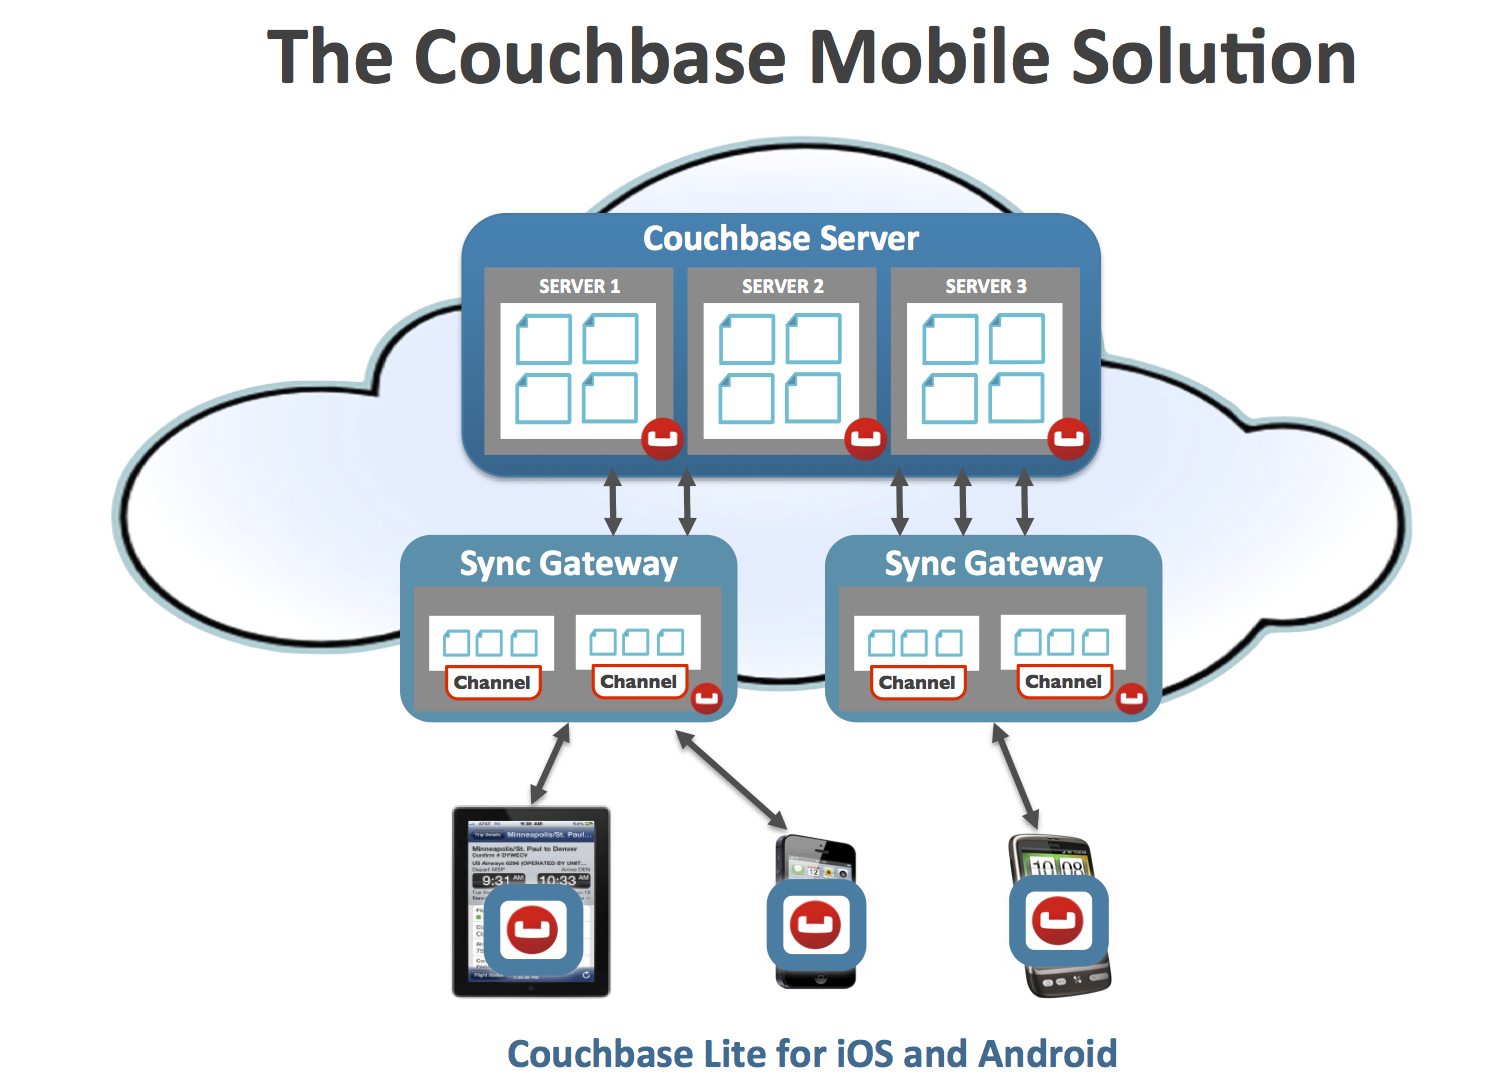
\includegraphics[width=1\linewidth]{./mobile-solution}
\caption[Architektur]{Architektur}
\label{fig:mobile-solution}
\end{figure}
\bibliography{ref}
\end{document}